\section{Zipf-like Distribution and Common Data Set}
%OS data
%user data: zipf
%prediction
%say something about aliyun
In Aliyun's VM cloud, each VM has one OS disk, plus one or more data disks.
During VM's ceation, its OS disk is directly copied from user's choosen base image.
Through its lifetime user may change configurations, install software, or write user data into OS disk,
but most of the OS and software related data shall keep unchanged. 
Previous study has also supported this\cite{vmimage}. Therefore, we can let all OS disks share these
common data in their snapshot backups.

Furthermore, our study on user's data disks has shown that the duplication pattern of
variable-sized data blocks follows \emph{Zipf-like} distribution. As a result, the major portion of 
deduplication effect will emerge from eliminating the duplication of frequently seen data.
%define CDS
\subsection{OS CDS}
We define \emph{OS CDS} to be the unchanged data across the base VM image and the snapshots of all
OS disks which are derived from it. Such data are brought by the operating system and popular 
software installations, they are rarely modified or deleted, and can be easily extracted using 
base image data as a hint.

To see the data duplication of OS CDS, we choose 7 major OSes in our VM cloud platform, which are:
Win2008 Server 64 bits, Win2003 Server 32 bits, Win2003 Server 64 bits, RHEL, CentOS, Ubuntu Server and Debian (all Linux
distributions are 64 bits).
Then we pick 5 VMs for each OS, and 10 snapshots for each VM. These VMs have been actively used by their
owners, their OS disks are heavily modified, some users even store huge amount of user data on
their OS disks. For example, some Ubuntu OS disks have only 2GB of data while some have 50GB.

We take the following steps to evaluate the effect of OS CDS: for each OS, the base image and all OS
disk snapshots are splitted into variable-sized blocks using TTTD algorithm. Then for every data block
in base image, we check if this block appear in all 50 snapshots. 

%table

The above analysis is only an estimation of OS and software related common data, 
some user installed software may not be discovered by this method because they are not included in the
base image. However, as we can see in the next section, the overall duplication of user generated data
follows the Zipf-like distribution, thus all popular data can be discovered by statistical analysis.

\subsection{Zipf-like Distribution and Data CDS}
Zipf's law has been shown to characterize use of words in a natural language, city populations, 
popularity of website visits and other internet traffic data.

Here we present the first fully consistent empirical study showing that data duplication
pattern in very large scale storage follows Zipf-like distribution. More specifically,
we show that the duplication count of any unique data block is inversely proportional to its rank
in the frequency table, with $\alpha$ smaller than unity. 
As far as we know, this is the first study of large scale real user data to disclose
the Zipf-like distribution pattern in data storage area.

\subsubsection{The model}
Consider a general storage system that holds user's files without any deduplication. 
Let $N$ be the total number of unique data blocks after 
content-defined chunking and deduplication, 
$C_N(i)$ be the number of duplicate copies that the $i$th data block being
stored in storage, given all the unique data blocks be ranked in order of their number of duplicate copies.
Let $S_i$ be the size of $i$th block,
then the actual ranking of the $i$th block is reflected by $\sum_{1}^{i-1}S_i$. 

\subsubsection{Methodology}
1323 users' virtual data disks were scanned using TTTD content-defined chunking, and we performed global perfect deduplication 
to caculate the number of duplicate copies of each individual unique block. We choose 2KB, 4KB, 16KB as the minimum, average
and maximum block size, all variable-sized blocks are compared by their SHA-1 hash arther than real data.

We choose user's data disks rather than OS disks in thie experiment for several reasons: First, the data in OS disks are 
instinctively highly similar, because most of the VM users only make some common or unique but tiny changes to their OSes,
so the data duplication pattern in OS disks cannot reflect the real distribution of general user data.
Second, the data disks are way more important in terms of data safty and backup because they are 
what users really care about.

\subsubsection{Result}
\begin{figure}
\centering
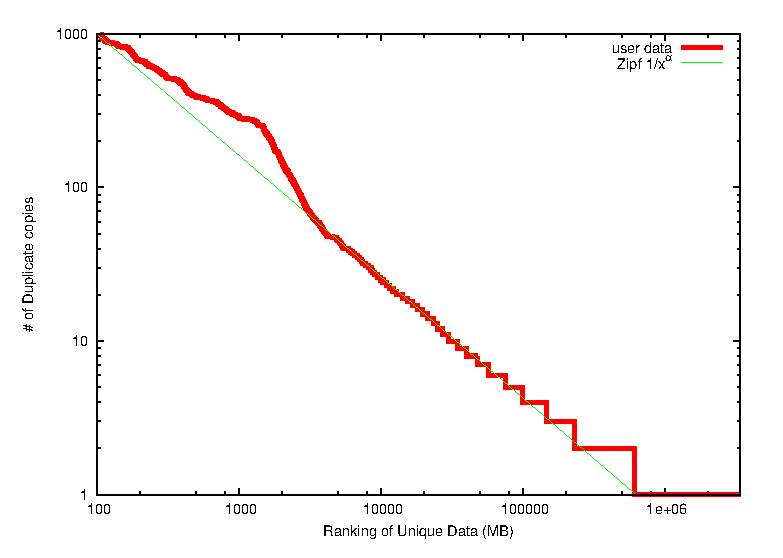
\epsfig{file=images/log-log.disk.eps, height=2in, width=2.66in}
\caption{Number of duplicate copies vesus block ranking}
\label{fig:zipf}
\end{figure}

Figure \ref{fig:zipf} shows the block duplication count vesus its ranking by that count. The almost straight line proves 
the block duplication in user generated data follows Zipf-like distribution, with $\alpha$ close to 0.78.
A tiny hottest fraction of data lead to majority of data duplication, as a result, we can target at this small set of commonly seen data
to design our fast and lightweight deduplication process, just like what people did in CDN and web proxy.

\subsection{Discussion}
By storing the hash index of a small set of hottest data (CDS), we expect to acheive great deduplication effect with minimal cost.
But one problem of the CDS is what we called \emph{blind spot}: the update of CDS is always behind new data's arrival,
as a result, some data must have been written to the backup store before being collected into CDS, thus such duplication may comprise the effect of
CDS. For instance, when a MySQL update is released, some users may apply it very quickly, so the new hot data bring by
this update will not be filtered by CDS. Only until later our CDS update includes those new data, then the rest of MySQL users get benefited.
We can take a few measurements to reduce the impact of blind spot. First, the data in blind spot will not accumulate, because snapshots backup
is a paid service, so over the long term, data in blind spot will be removed from backup store as VMs and old snapshots keep being deleted.
Second, for the major OS updates, we can anticipate them in advance by putting the new hot data into CDS before users widely adopt them.

Another problem associated with CDS is that some data in CDS may no longer be popular or even disappear
as time goes. For example, an MySQL software update may invalidate some data that we previously hold in 
the CDS. If some data blocks in CDS are no longer referenced, our map-reduce process is able to detect
this situation, so invalid data will be removed and new data will be added during the next CDS update. 
But if some users choose to keep their old MySQL version, then the corresponding old and new data will co-exist in the CDS.
